\documentclass[portrait,final]{pmposter}

% Folder(s) where LaTex is supposed to search for figures.
\graphicspath{{figures/}}

\usepackage{amsmath}
\usepackage{bookman}
\usepackage{float}
\usepackage{lipsum}

\newcommand{\screenid}{1}
\newcommand{\posterid}{0}

% Title, authors and affiliations.
\title{A Wonderful Placeholder Poster---screen \screenid{}, poster \posterid}
\author{Luca Baldini}
\affil{Universit\`a and INFN-Pisa}

\begin{document}

\begin{poster}
  { % Poster Options---change stuff at your leisure.
    grid            = no             , % Visualize a debug grid.
    headerheight    = 0.22\textheight, % The height of the title/author block.
    titlefont       = \bf\huge       , % Font for the title.
    authorfont      = \large         , % Font for the authors/affiliations.
    abstractfont    = \large         , % Font for the abstract box.
    headerfont      = \bf\Large      , % Font for the box headers.
    textfont        = \normalsize    , % Font for the body text.
    textmargin      = 0.5em          , % Left/right margins for the body text.
    textcolor       = nicegray           , % Default text color.
    twocolsabstract = no             , % Use two columns for the abstract.
    linewidth       = 2pt              % Width of the lines.
  }
  { % Logo.
    \includegraphics[width=0.6\textwidth]{fdfp}
  }
  {}


  \abstract{Placeholder poster for the 15th Pisa Meeting on Advanced Detectors}{
    This is a simple placeholder to debug the poster display system for the
    forthcoming Pisa Meeting on Advanced Detectors.
  }


  % If you specify the height, that's relative to the poster height, i.e., 0.3
  % is 30% of the poster). If you don't the box will adapt itself to the content.
  \headerbox{Text}{name=textbox,column=0,span=3, below=abstract, height=0.4}
  {
    Sample box for plain text. You will notice that we have deliberately chosen
    a font that is hard to read.

    \bigskip

    And, for completeness, here are different font sizes:
    \begin{itemize}
    \item {\Huge this text is Huge;}
    \item {\huge this text is huge;}
    \item {\LARGE this text is LARGE;}
    \item {\Large this text is Large;}
    \item {\large this text is large;}
    \item this text is normal;
    \item {\small this text is small;}
    \item {\footnotesize this text is footnotesize;}
    \item {\scriptsize this text is scriptsize;}
    \item {\tiny this text is tiny;}
    \end{itemize}

    Cool, isn't it?
  }

  \headerbox{Graphics}{name=graphbox,column=0, span=3, below=textbox, height=0.48}
  {
    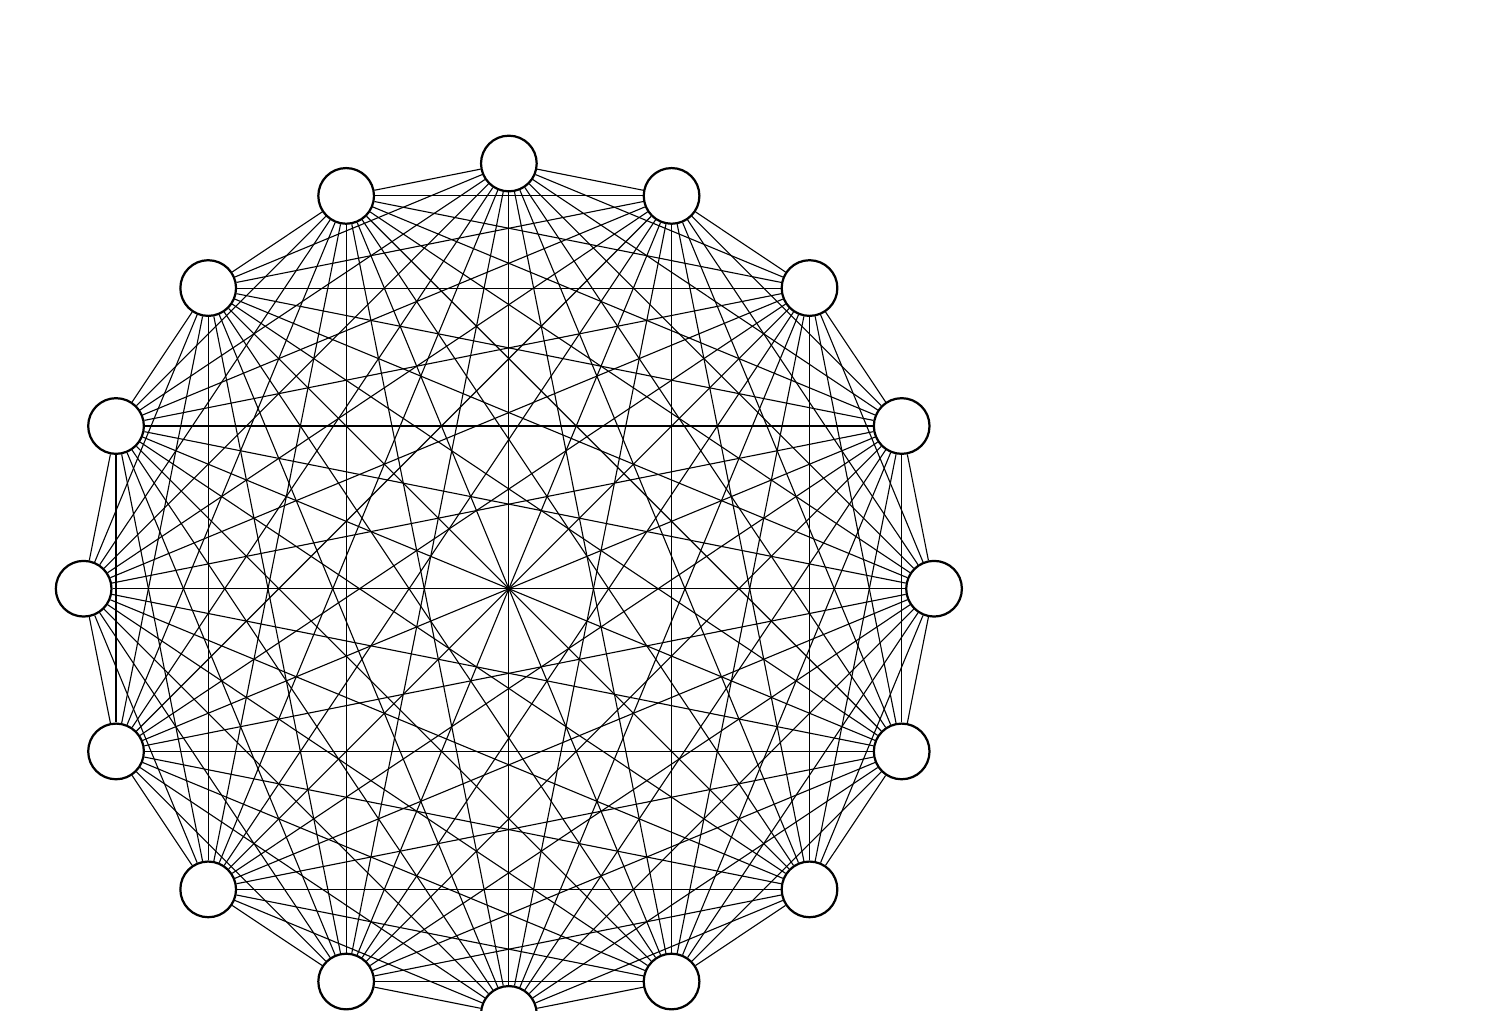
\begin{tikzpicture}[x=\linewidth, y=\linewidth]%
      \useasboundingbox (-0.504, 0) rectangle (1., 1.);%
      \foreach \x in {1,...,16}{%
        \pgfmathparse{(\x-1)*45 + floor(\x/9)*22.5}
        \node[draw,circle,inner sep=0.25cm,yshift=5.cm] (N-\x) at (\pgfmathresult:5.4cm) [thick] {};
      }
      \foreach \x [count=\xi from 1] in {2,...,16}{%
        \foreach \y in {\x,...,16}{%
        \path (N-\xi) edge[-] (N-\y);
      }
    }
    \end{tikzpicture}
  }

  \headerbox{Pictures}{name=picbox, column=3,span=3, below=abstract, height=0.35}
  {
    How does this look like?

    \medskip

    \begin{figure}[H]
      \includegraphics[width=\linewidth]{cms_tracker}
      \caption{The CMS silicon tracker (courtesy of CERN).}
    \end{figure}
  }


  \headerbox{Miscellanea}{name=miscbox,column=3,span=3, below=picbox, height=0.37}
  {
    \lipsum[3-4]
  }

  \bibbox{name=referencebox,column=3,span=3,below=miscbox, bottomaligned=graphbox}{
  \bibitem{p8dwarfs} Ackermann, M. et al, \emph{Searching for Dark Matter Annihilation from Milky Way Dwarf Spheroidal Galaxies with Six Years of Fermi-LAT Data}, \texttt{arXiv:1503.02641}, accepted for publication on PRL
  }

\end{poster}

\end{document}
